\documentclass{article}
\usepackage[T1]{fontenc}
\usepackage{lmodern}
\usepackage{graphicx}
\usepackage{amsmath,amssymb}
\usepackage[a4paper,margin=2cm]{geometry}
\usepackage[absolute,overlay]{textpos}
\setlength{\TPHorizModule}{1mm}
\setlength{\TPVertModule}{1mm}
\usepackage[indonesian]{babel}
\usepackage{hyperref}
\setlength{\emergencystretch}{2em}
% unit: Halaman 50

\begin{document}

% === Halaman 50 (llm) ===

% (tidak ada teks dari model)

% deskripsi: Tabel yang membandingkan berbagai mode operasi cipher termasuk ECB, CBC, CFB, OFB, dan CTR, mencakup deskripsi dan aplikasi tipikal masing-masing.
% bbox normalisasi: [0.1400, 0.7000, 0.8100, 0.9030]
\begin{textblock*}{140.70mm}(29.40mm,207.90mm)
\noindent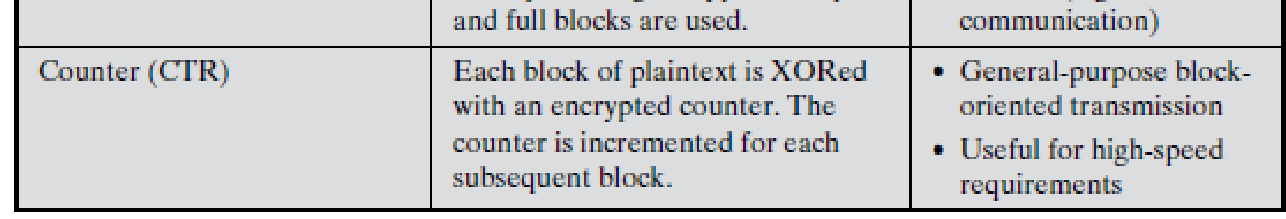
\includegraphics[width=140.70mm,height=60.29mm]{../../images/llm/page_050_img_01.png}%
\end{textblock*}

\end{document}
